\section{Results and sensitivity analysis}\label{results}
This section presents the most relevant quantitative results of the proposed case study. Section \ref{res:district_heating} elaborates on the district heating option in the \textit{Directed Transition} scenario. Section \ref{res:heat_pump} focuses on the implementation of a heat pump system in the \textit{Societal Commitment} scenario where the model indicates feasible solutions for a retrofitted building with lower heat demand only (compared to the default settings). A comparison of the results of the district heating and heat-pump-based heat supply in the different scenarios quantified in this work is conducted in Section \ref{res:overview}. Finally, Section \ref{res:co2_shares} presents the results in case of varying CO\textsubscript{2} pricing cost allocation between the landlord as the building owner and the tenants. 

\subsection{District heating in the Directed Transition scenario}\label{res:district_heating}
Following up Table \ref{tab:values} in Section \ref{sec:data}, this section presents the results of the district heating implementation in the \textit{Directed Transition} scenario in detail. Figure \ref{fig:dt+dh} shows the net present value of cash flows in general, and revenues in particular, of the landlord and a single tenant within the time horizon $2025$ to $2040$. Figure \ref{fig:dt+dh} (top left) presents the different items of the landlord consisting of the overnight investment costs (light blue), investment grant (blue), and rent-related revenues (yellow). Note that latter represent the additional rent-related revenues due to the newly installed sustainable heating system. Figure \ref{fig:dt+dh} (bottom left) shows the development of the landlord's net present value of its cashflow over time. Thereby, it is shown that the investment pays off for the landlord by zero in $2040$. The two Figures \ref{fig:dt+dh} (top right, bottom right) illustrate the corresponding tenant's cash flow items (top) and total net present value (bottom) until $2040$. 

\begin{figure}[h]
	\centering
	\includegraphics[width=0.9\linewidth]{figures/4_Results/fig_DT_DH/detail.eps}
	\caption{Development of the landlord's and tenant's economic viability of the district heating option in the \textit{Directed Transition} scenario. Top left: landlord's cash flows, bottom left: landlord's net present value, top right: tenant's cash flows, bottom right: tenant's net present value}
	\label{fig:dt+dh}
\end{figure}

 The tenant receives subsidy payments from the governance between 2025 and 2030. Thus, the tenant's net present value in $2040$ matches with the value as in the reference case. The reference case considers constant remaining rent-related and heat-related costs for the tenant based on the initial rent, gas-based heat system parameters, and CO\textsubscript{2} prices as of 2025. In the years 2025 to 2029, the subsidy payments exceed the heating costs of the tenant. Note that the tenant already pays a higher rent charge to the landlord within the same period (see the yellow bars in Figure \ref{fig:dt+dh} top left). Most importantly, the tenant's reference net present value ("Ref. (Gas/2025)"; gray dashed line in the Figure \ref{fig:dt+dh} bottom right) shows a crucial aspect of the results and assumptions of the analysis which requires an explanation. Since "Ref. (Gas/2025)" is used as the initial tenant's spendings, the results also take into account the total opportunity costs (i.e., those costs that would be incurred by sticking to the initial gas-based heating system for the tenant due to a rising CO\textsubscript{2} price). Note that the openENTRANCE decarbonization scenarios used in this work do consider both a significant increase of the CO\textsubscript{2} price and a decrease of the specific emissions of the district heating and electricity fueling mix. The quantitative results indicate that the heating system change in this scenario is achieved with manageable total governance's subsidies. However, a detailed discussion of the allocation of CO\textsubscript{2} price-related opportunity costs is conducted in Section \ref{res:co2_shares}.

\subsection{Heat pump and building stock quality in the Societal Commitment scenario}\label{res:heat_pump}
Interestingly, the model indicates for the heat pump implementation in the \textit{Societal Commitment} scenario an infeasible solution. The reason for that is, among others (investment costs of the air-sourced heat pump and the electricity price) the high heating demand used in the default input settings. Therefore, in the following the focus is put on the impact of different building renovation levels, the associated heating demand decrease, and finally the impact on the feasibility of the model.\vspace{0.5cm} 

Figure \ref{fig:retrofitting} shows the results of the heat pump implementation in the \textit{Societal Commitment} scenario for four different building quality (and thus heat demand levels) in detail. Since the initial setting of the default building in terms of total and peak heat demand leads to the infeasibility of the model, the following three additional renovation levels are studied: \SI{10}{\%}, \SI{20}{\%}, and \SI{30}{\%} reduction of both the total and peak heat demand. In Figure \ref{fig:retrofitting} (top left) the corresponding settings of the specific heat load (describing building quality) are indicated.

\begin{figure}[h]
	\centering
	\includegraphics[width=0.9\linewidth]{figures/4_Results/fig_retrofitting/retrofitting.eps}
	\caption{Comparison of the heat pump option in the \textit{Societal Commitment} scenario for different renovation levels. Top left: governance's objective value, top right: landlord's investment grant, bottom left: tenant's subsidy payment per unit, bottom right: landlord's rent-related revenues in total}
	\label{fig:retrofitting}
\end{figure}

In case of a \SI{10}{\%} reduction of the heat demand, the landlord receives a significant investment grant be equivalent to \SI{29}{\%} of the landlord's total overnight investment costs of the building retrofitting measures (Fig. \ref{fig:retrofitting} top right). The associated tenant's subsidy payment takes place between 2025 and 2030 with a maximum of \SI{2~040}{EUR \per year} (Fig. \ref{fig:retrofitting} bottom left). The rent charge adjustment and related revenues remain almost constant during the period (Fig. \ref{fig:retrofitting} bottom right). In case of a \SI{20}{\%} reduction of the heat demand, the landlord receives only a small investment grant related to the total overnight investment costs (\SI{2}{\%}). The tenant's subsidy payment takes place between 2025 and 2032 with a maximum of \SI{2~556}{EUR \per year}. The landlord's rent-related revenues increase until 2031 and then remain constant. In case of a \SI{30}{\%} reduction of the heat demand, the landlord receives as before a small investment grant (\SI{3}{\%}). Instead, the landlord makes significant rent-related revenues (the highest among the three renovation levels). The tenant gets subsidy payments in most years, excluding 2026 and 2028 to 2030 (mainly as a result of the matching of the CO\textsubscript{2} price and the specific CO\textsubscript{2} emissions of the fueling energy mix). The maximum is \SI{2~796}{EUR \per year} in 2040. The lower heat energy-related costs as a result of the building renovation lead to higher rent charge payments. Hence, smaller investment grants supporting the landlord are sufficient. 

\subsection{Governance's total subsidies in the different scenarios}\label{res:overview}
In this section, a comparison of the governance's total subsidies for district heating (DH) or heat pump (HP) implementation in the different scenarios is conducted. Table \ref{tab:objective} and Figure \ref{fig:npv_comparison} present the quantitative result of this comparison. In summary, the following interesting observations are made:

\begin{itemize}
	\item The total subsidies across the three district heating cases are relatively stable and are within \SI{11.2}{\%}.
	\item The heat pump implementation in the two decarbonization scenarios \textit{Societal Commitment} and \textit{Gradual Development} is infeasible for the default setting of the building quality (see discussion already in Section \ref{res:heat_pump}).
	\item Only the low CO\textsubscript{2} price development scenario provides a solution for the heat pump but with a significantly higher subsidy +\SI{82.6}{\%} compared to the lowest subsidy scenario.
\end{itemize}

\definecolor{Gray}{gray}{0.95}
\begin{table}[h]
	\centering
	\scalebox{0.8}{
		\renewcommand{\arraystretch}{1.35}
		\begin{tabular}{lcccccc}
			\toprule 
			& \multicolumn{3}{c}{District heating (DH)} & \multicolumn{3}{c}{Heat pump (HP)}\\
			\cmidrule(lr){2-4}\cmidrule(lr){5-7}
			\multirow{2}{*}{Governance's total financial support}& DT & GD & LD & SC & GD& LD\\
			\cmidrule(lr){2-2}\cmidrule(lr){3-3}\cmidrule(lr){4-4}\cmidrule(lr){5-5}\cmidrule(lr){6-6}\cmidrule(lr){7-7}
			& (\SI{1.5}{\degreeCelsius}) & (\SI{2.0}{\degreeCelsius}) & (-) & (\SI{1.5}{\degreeCelsius}) &  (\SI{2.0}{\degreeCelsius}) & (-)\\
			\hline
			Absolute in thous. \SI{}{EUR} & \SI{211.4}{} & \SI{195.5}{} & \cellcolor{Gray}\SI{190.1}{} & \textit{infeasible} & \textit{infeasible} & \SI{351.5}{}\\
			Rel. change in \% of LD (DH) & \SI{11.2}{} & \SI{2.6}{} & - &  & & \SI{82.6}{}\\ 
			\bottomrule
	\end{tabular}}
	\caption{Comparison of governance's total financial support for the different heating system alternatives and scenarios (explanations of shortcuts in Table \ref{tab:scenarios})}
	\label{tab:objective}
\end{table}

When comparing Table \ref{tab:objective} and Figure \ref{fig:npv_comparison} it is important to note that the landlord's rent-related revenues (orange bar) are an "implicit" subsidy. Hence, the total governance's total financial support are equal to the sum of the tenants' heating costs subsidy (purple bar) and the landlord's investment grant (blue bar). 

\begin{figure}[h]
	\centering
	\includegraphics[width=0.65\linewidth]{figures/4_Results/fig_npv_comparison/net_present_value.eps}
	\caption{Comparison of governance's total financial support for the landlord and the tenants for district heating (DH) and heat pump (HP) implementation in the different scenarios}
	\label{fig:npv_comparison}
\end{figure}

\subsection{Allocation of CO\textsubscript{2} pricing related costs between the governance, landlord and tenant}\label{res:co2_shares}
This section examines the impact of the costs of inaction (i.e., sticking to the initial gas-based heating system) on the governance's total financial support. In detail, this means the CO\textsubscript{2} costs (i.e., opportunity costs) to be expected due to increasing CO\textsubscript{2} prices have to be allocated to the different parties/agents (or a single one): governance, landlord, and tenant. Table \ref{tab:allocation} provides an overview of the different cases on the allocation of the opportunity cost (i.e., CO\textsubscript{2} costs of inaction) compared to the alternative on district heating implementation in the \textit{Gradual Development} scenario.

\definecolor{Gray}{gray}{0.95}
\begin{table}[h]
	\centering
	\scalebox{0.85}{
		\renewcommand{\arraystretch}{1.2}
		\begin{tabular}{lccc}
			\toprule
			Rel. allocation of opportunity costs& Governance & Landlord & Tenants\\
			\hline
			Case A (equally) & $\frac{1}{3}$ & $\frac{1}{3}$ & $\frac{1}{3}$\\
			Case B (landlord \& tenant) & 0 & $\frac{1}{2}$ & $\frac{1}{2}$\\
			Case C (landlord) & 0 & $1$ & 0\\
			Case D (governance \& tenant) & $\frac{1}{2}$ & 0 & $\frac{1}{2}$\\
			\hline
			\cellcolor{Gray}Scenarios from Sec. \ref{sec:scenarios} (governance)& \cellcolor{Gray}$1$ & \cellcolor{Gray}0 & \cellcolor{Gray}0\\
			\bottomrule
	\end{tabular}}
	\caption{Allocation of the CO\textsubscript{2}-related opportunity costs (costs of inaction) among the governance, the landlord, and tenants}
	\label{tab:allocation}
\end{table}


Exemplarily, "Case A (equally)" takes into account that the CO\textsubscript{2} costs are shared equally among the governance, landlord, and tenants. Each of them bear one third of the costs. Note that the scenario setups from Section \ref{sec:scenarios} considered so far that the total costs of inaction are covered by the governance (see Equation \ref{c:ten2} and \ref{c:ten4}). The mathematical formulation of the modifications here in this section can be found in \ref{app:varying}. Figure \ref{fig:3dplot} presents the results of the varying allocation of the opportunity costs. The metric used is the relative change of the objective value (i.e., governance's total subsidies). The objective value of the district heating option in the \textit{Gradual Development} scenario (GD (DH)) is used as the reference value and marked by the black point in the upper left corner in Figure \ref{fig:3dplot}. The negative signs indicate that the consideration of the costs associated with the withdrawal of the problem (i.e., CO\textsubscript{2} price related opportunity costs) results in a reduction of the necessary governace's total subsidies.

\begin{figure}[h]
	\centering
	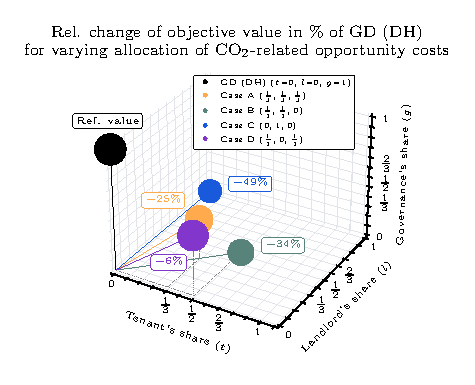
\includegraphics[width=0.75\linewidth]{figures/4_Results/fig_3d_plot/3d.eps}
	\caption{Comparison of the objective value for varying allocation of opportunity cost among the tenants (x-axis), the landlord (y-axis), and governance (z-axis) switching to district heating. The size of the points corresponds to the objective function value in proportion to the \textit{Gradual Development scenario} (percentage change in the boxes).}
	\label{fig:3dplot}
\end{figure}

Most importantly, the highest total subsidy reduction is obtained in "Case C" where the landlord has to cover the costs of inaction (-\SI{49}{\%} compared to the reference value). The second highest reduction is in "Case B". In this case, the opportunity costs are shared equally within the building among the landlord and tenants (-\SI{34}{\%}). "Case A" reduces the total subsidy by \SI{25}{\%}.  It is evident that an even allocation between the governance and the tenants ("Case D") hardly leads to a reduction of the objective value. The main reason for this is the financial support of the landlord, which is necessary to create an investment incentive, and the fact that the finacial support between the landlord and tenants necessarily has the same net present value.\vspace{0.5cm}

Eventually, Figure \ref{fig:feasible} shows the objective value for varying landlord's interest rates. Note that these results are located in the YZ-plane spanned by the landlord's and governance's share in the costs of inaction in Figure \ref{fig:3dplot}. Particularly, "Ref. value" (black, Fig. \ref{fig:3dplot}) and "Case B" (dark blue, Fig. \ref{fig:3dplot}) specify the two endpoints of the blue line in Figure \ref{fig:feasible} with $i_l=\SI{10}{\%}$. 

\begin{figure}[h]
	\centering
	\includegraphics[width=0.7\linewidth]{figures/4_Results/fig_feasible/feasible.eps}
	\caption{Comparison of the objective value for varying landlord's interest rates and share in costs of inaction}
	\label{fig:feasible}
\end{figure}

The varying landlord's interest rates have two important impacts. First, a decreasing interest rate reduces the objective value as revenues are discounted less (see Fig. \ref{fig:feasible} for a fixed landlord's share in costs of inaction, e.g., $0.2$). Second, as the interest rate decreases, a feasibility limit becomes apparent. This means, that the feasible maximum of the landlord's share in costs of inaction depends on the landlord's interest rate $i_l$ (e.g., \SI{100}{\%} for $i_l=\SI{10}{\%}$, \SI{70}{\%} for $i_l=\SI{5}{\%}$ and \SI{60}{\%} for $i_l=\SI{3}{\%}$). Two interesting energy policy implications can be derived from the results here:
\begin{itemize}
	\item In case the landlord is very much profit oriented (e.g., interest rate of $\SI{10}{\%}$) and governance's total subsidy payments are to be kept as low as possible, complete allocation of the CO\textsubscript{2}-related opportunity costs to the landlord results in a cost-optimal strategy.
	\item In contrast, in case the landlord serves rather a public-benfit purpose (e.g., interest rate of $\SI{3}{\%}$), the CO\textsubscript{2}-related opportunity costs allocation among governance, landlord, and tenants is an adequate strategy.
\end{itemize}


